% 2012
% Maciej Szeptuch
% II UWr

\documentclass[11pt,leqno]{article}

\usepackage[utf8]{inputenc}
\usepackage{polski}
\usepackage{a4wide}
\usepackage[cm]{fullpage}

\usepackage{graphicx}
\usepackage{epstopdf}
\usepackage{amsmath,amssymb}
\usepackage{bm}
\usepackage{amsthm}

%% Kropka po numerze paragrafu, podparagrafu, itp.
\makeatletter
    \renewcommand\@seccntformat[1]{\csname the#1\endcsname.\quad}
    \renewcommand\numberline[1]{#1.\hskip0.7em}
\makeatother

%% Numeracja wzorów
\renewcommand{\theequation}{\arabic{section}.\arabic{equation}}

%%%%%%%%%%%%%%%%%%%%%%%%%%%%%%%%%%%%%%%%%%%%%%%%%%%%%%%%%%%%%%%%%%%%%%%%%%%%%%%%

\title{\LARGE \textbf{{Pracownia z analizy numerycznej}}\\
      {\Large Sprawozdanie do zadania \textbf{P2.17.}}\\
      {\large Prowadzący: dr Paweł Woźny}
}
\author{Maciej Szeptuch}
\date{Wrocław, \today}

\begin{document}
\thispagestyle{empty}
\maketitle

%%%%% WSTĘP
\section{Wstęp - Interpolacja wielomianowa}\label{S:Wstęp}
Interpolacja wielomianowa jest metodą numeryczną przybliżania funkcji tzw.
wielomianem Lagrange'a stopnia n, przyjmującym w n+1 punktach, zwanych
węzłami interpolacji wartości takie same jak przybliżana funkcja.
Stosowana jest gdy dysponuje się skończoną liczbą danych do określenia
zależności między wielkościami oraz w celu uproszczenia skomplikowanych
funkcji, np. podczas całkowania numerycznego.\\
W zadaniu mamy dane trzy następujące różne postacie wielomianów interpolujących
w punktach charakterystycznych wielomianów Czebyszewa.\\
Wielomian $I_n$ interpolujący f w węzłach Czebyszewa $t_{n+1,k}$ \eqref{E:Wezly}:
\begin{equation}
    I_n(x) = \frac{2}{n+1}\sum_{i=0}^{n}'\Big(\sum_{j=0}^nf(t_{n+1,j})T_i(t_{n+1,j})\Big)T_i(x)
\end{equation}
Wielomian $J_n$ interpolujący f w ekstremach wielomianu Czebyszewa $u_{n,k}$\eqref{E:Ekstrema}:
\begin{equation}
    J_n(x) = \frac{2}{n}\sum_{j=0}^{n}''\Big(\sum_{k=0}^n''f(u_{n-1,k})T_k(u_{n-1,j})\Big)T_j(x)
\end{equation}
$n-$ty wielomian optymalny w sensie aproksymacji jednostajnej:
\begin{equation}
    K_n(x) = \frac{2}{n+1}\sum_{j=0}^{n}'\Big(\sum_{k=0}^n''f(u_{n,k})T_k(u_{n,j})\Big)T_j(x)
\end{equation}
gdzie:
\begin{equation}\label{E:Wezly}
    t_{n+1,k} = \cos\frac{2k+1}{2n+2}\pi \qquad\mbox{($k = 0,1,...,n$)}
\end{equation}
\begin{equation}\label{E:Ekstrema}
    u_{n,k} = \cos(k\pi/(n+1)) \qquad\mbox{($k = 0,1,...,n+1$)}
\end{equation}
W doświadczeniu przyjęto za $f$ funkcje wykładniczą $e^x$, trygonometryczną $\sin x$
oraz wielomian stopnia 10 z losowymi współczynnikami. Interpolacje zastosowano dla $n = 1, 4, 7, 10$.

\section{Podstawy teoretyczne}
\subsection{Wielomiany Czebyszewa}\label{SS:Czebyszew}
Są to wielomiany, nazwane po Pafnutiju Czebyszewie, które spełniają równanie rekurencyjne:
\begin{equation}\label{E:Czebyszew}
    T_0(x)=1\ T_1(x)=x\ T_k(x)=2x\cdot T_{k-1}(x) - T_{k-2}(x)
\end{equation}
Mają one szerokie zastosowanie między innymi w interpolacji wielomianowej. Użycie jako węzłów zer tych wielomianów pozwala uniknąć tak zwanego efektu Rungego, czyli dużych błędów interpolacji przy końcach przedziału.

\subsection{Aproksymacja jednostajna}\label{SS:Aproksymacja}
Aproksymacja, czyli przybliżanie(w tym przypadku wartości funkcji), której celem jest minimalizacja największego błędu. Można go przedstawić w postaci:
$$
    E = \max_{x\in[a,b]}|g(x)-f(x)|
$$
gdzie $f(x)$ to przybliżana funkcja a $g(x)$ to obliczone przybliżenie w x.

\subsection{Algorytm Clenshawa}\label{SS:Clenshaw}
Do obliczenia wartości wielomianów interpolacyjnych oraz ich współczynników został użyty algorytm Clenshawa. Jest to algorytm, który można wykorzystać do obliczania sum $S_n(x) = \sum_{k=0}^{n}c_kF_k(x)$, czyli takich jakie mamy w zadaniu.\\
W ogólności jest on określony dla ciągu wielomianów $F_n$ spełniających warunki:
$$ F_0(x) = \alpha_0, F_1(x) = (\alpha_1 x - \beta_1)F_0(x), $$
$$ F_k(x) = (\alpha_k x - \beta_k)F_{k-1}(x) - \gamma_k F_{k-2} \qquad\mbox{($k = 2, 3, ...$)} $$
gdzie $\alpha_k$, $\beta_k$ oraz $\gamma_k$ są określonymi ciągami współczynników. \\
Algorytm ten polega na obliczaniu wielkości $B_k$ ($k=0,1,...,n+2$) według wzorów:
$$ B_{n+1} = B_{n+2} = 0 $$
$$ B_k = c_k + (\alpha_{k+1} x - \beta_{k+1})B_{k+1} - \gamma_{k+2}B_{k+1} \qquad\mbox{($k=n,n-1,...,0$)} $$
A wynikiem jest: $S_n = \alpha_0B_0$.\\ \\
W przypadku tego zadania, gdzie pojawiają sie kombinacje postaci:
$$
    \frac{c_0}{2} + c_1T_1(x) + c_2T_2(x) + ... + c_nT_n(x)
$$
Algorytm ten przyjmuje prostą postać:
$$ B_{n+1} = B_{n+2} = 0 $$
$$ B_k = c_k + 2xB_{k+1} - B_{k+2} \qquad\mbox{($k=n,n-1,...,0$)} $$
z wynikiem:
$$ S_n(x) = \frac{1}{2}[B_0 - B_2] $$
\section{Doświadczenie}\label{S:Doświadczenie}
Korzystając z podanych wzorów, obliczając odpowiednie wartości za pomocą algorytmu Clenshawa,
obliczono odpowiednie wielomiany interpolujące i przybliżono ich błąd w sensie aproksymacji
jednostajnej. Do obliczeń wykorzystano program w C++\footnote{program.cpp w prog/}, używając double dla
obliczeń podwójnej precyzji. Współczynniki dla wielomianów $J_n$ oraz $K_n$ zostały obliczone przy pomocy algorytmu Clenshawa. Dla $I_n$ współczynniki zostały obliczone przy pomocy tabelki kwadratowej $l_{i,j} = f(t_{n+1,j})T_i(t_{n+1,j})$ z której następnie zsumowano odpowiednie wiersze aby otrzymać potrzebne wartości. Ostateczne wartości wszystkich wielomianów były już obliczane przy pomocy Clenshawa z użyciem tych współczynników.
\subsection{Funkcja wykładnicza $e^x$}
Jak możemy zauważyć na wykresach \eqref{G:Wykresex4} i \eqref{G:Wykresex7}, funkcje wykładniczą najlepiej, prawie identycznie do siebie, przybliżają wielomiany $I_n$ oraz $K_n$. Błąd $J_n$ jest niemal dwa razy większy niż dwóch pozostałych, co możemy lepiej zaobserwować porównując wartości błędów z tabeli.
\begin{center}
    \begin{tabular}{r|l|l|l}
        \texttt{$n$} & \texttt{błąd $I_n$} & \texttt{błąd $J_n$} & \texttt{błąd $K_n$} \\ \hline
        $1$ & $0.369064391011796999$ & $0.557602907747600129$ & $\textbf{0.286062590339978273}$ \\
        $4$ & $0.000617655698656794$ & $0.001065951594156456$ & $\textbf{0.000550086046028797}$ \\
        $7$ & $0.000000220402020634$ & $0.000000397373810079$ & $\textbf{0.000000200429180808}$ \\
        $10$ & $0.000000000027039260$ & $0.000000000049913851$ & $\textbf{0.000000000025064839}$ \\
    \end{tabular}
\end{center}
\subsection{Funkcja trygonometryczna $\sin x$}
W przypadku sinusa sytuacja jest interesująca, na wykresach \eqref{G:Wykressin4} oraz \eqref{G:Wykressin7} możemy zauważyć, że wielomiany $K_n$ oraz $I_n$ nie są już cały czas tak podobne do siebie, ale ich błędy w sensie jednostajnym nadal są zbliżone. Ciekawie wygląda sytuacja dla $J_n$, jego błąd potrafi być, tak jak w poprzednim przypadku, dwa razy większy ale możemy zauważyć, że np. dla $n = 1, 7$ jest nieznacznie lepszy niż wielomian $K_n$. Wynika to najprawdopodobniej z błędów zaokrągleń obliczeń zmiennoprzecinkowych. Warto jeszcze wspomnieć o kształcie wykresu, mimo że $K_n$ ma najmniejszą wartość błędu w sensie jednostajnym to $I_n$ oraz $J_n$ znacznie lepiej przybliżają sinus w okolicach $0$.
\begin{center}
    \begin{tabular}{r|l|l|l}
        \texttt{$n$} & \texttt{błąd $I_n$} & \texttt{błąd $J_n$} & \texttt{błąd $K_n$} \\ \hline
        $1$ & $0.077254385057671904$ & $\textbf{0.059993695411950931}$ & $0.059993695411950987$ \\
        $4$ & $0.000504385491298220$ & $0.000930285262303543$ & $\textbf{0.000499532757772925}$ \\
        $7$ & $0.000000020949158408$ & $\textbf{0.000000020490088404}$ & $0.000000020639655263$ \\
        $10$ & $0.000000000024034580$ & $0.000000000047404164$ & $\textbf{0.000000000023959945}$ \\
    \end{tabular}
\end{center}
\subsection{Wielomian stopnia 10 $x + 18x^2 + 2x^3 + 0.66x^5 + 0.167x^8 + 0.5x^9 + 0.125x^{10}$}
Również i w tym przypadku $K_n$ najlepiej przybliża w sensie jednostajnym, prawie dwa razy lepiej niż pozostałe wielomiany. Tak jak poprzednio jednak warto zwrócić uwagę na to że mimo iż $K_n$ jest najlepszy w sensie jednostajnym, to w przedziale od $-1$ do $0.5$ wielomian $I_n$ radzi sobie mniej więcej dwa razy lepiej.
\begin{center}
    \begin{tabular}{r|l|l|l}\label{T:Tabelapoly}
        \texttt{$n$} & \texttt{błąd $I_n$} & \texttt{błąd $J_n$} & \texttt{błąd $K_n$} \\ \hline
        $1$ & $11.141650402092894367$ & $18.429355494992332609$ & $\textbf{9.283355494992335366}$ \\
        $4$ & $0.191089364188730571$ & $0.214736695802418165$ & $\textbf{0.128290195991251466}$ \\
        $7$ & $0.007704961684876110$ & $0.009705010232415212$ & $\textbf{0.005469431638421951}$ \\
        $10$ & $0.000000000000053291$ & $0.000000000000019540$ & $\textbf{0.000000000000015987}$ \\
    \end{tabular}
\end{center}
\section{Wnioski}\label{S:Wnioski}
Jak możemy zauwazyć na podstawie przeprowadzonych doświadczeń, wielomian $K_n$ jest, tak jak być powinien, najlepszym wielomianem w sensie jednostajnym. Ale w przypadku kiedy zależy nam na pewnych szczególnych przedziałach argumentów wielomiany $I_n$ oraz $J_n$ mogą okazać się lepszym wyborem, ich przybliżenia mimo, że nie są najlepsze na całym przedziale to już w pewnym mniejszym zakresie mogą takie być, natomiast $K_n$ oscyluje cały czas w okolicach swojego maksymalnego błędu.
\thispagestyle{empty}
\begin{thebibliography}{99}
    \bibitem{Not} S. Lewanowicz, \textit{Notatki do wykładu z analizy numerycznej}, Wrocław, 2012r.
    \bibitem{Zas} S. Paszkowski, \textit{Zastosowania numeryczne wielomianów i szeregów Czebyszewa}, PWN, Warszawa, 1975r.
    \bibitem{Cle} \textit{Algorytm Clenshawa}, https://en.wikipedia.org/wiki/Clenshaw\_algorithm
    \bibitem{Cze} \textit{Wielomiany Czebyszewa}, https://en.wikipedia.org/wiki/Chebyshev\_polynomials
\end{thebibliography}
\thispagestyle{empty}
\begin{center}
    \begin{figure}[!ht]
        \begin{center}
        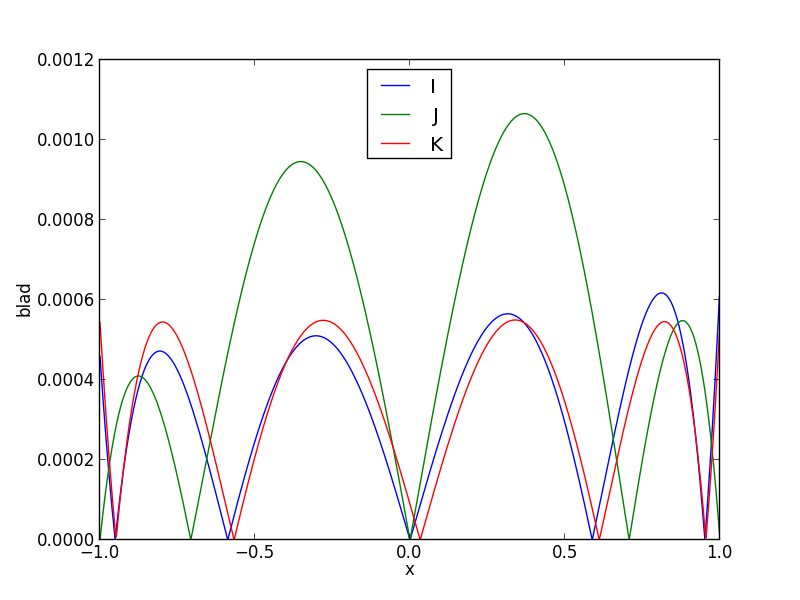
\includegraphics{graph0_4.png}
        \caption{Błąd bezwględny aproksymacji $e^x$ dla $n=4$}\label{G:Wykresex4}
    \end{center}
    \end{figure}
\end{center}

\begin{center}
    \begin{figure}[!ht]
        \begin{center}
        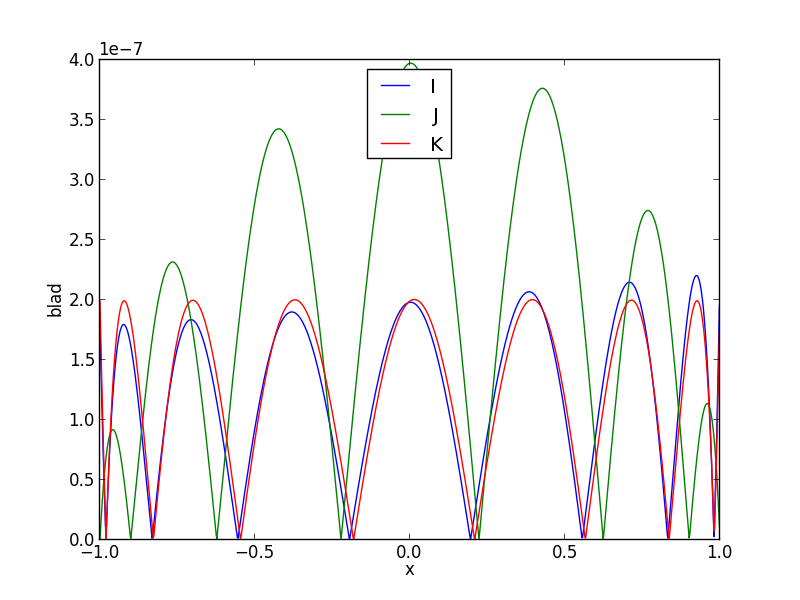
\includegraphics{graph0_7.png}
        \caption{Błąd bezwględny aproksymacji $e^x$ dla $n=7$}\label{G:Wykresex7}
    \end{center}
    \end{figure}
\end{center}
\begin{center}
    \begin{figure}[!ht]
        \begin{center}
        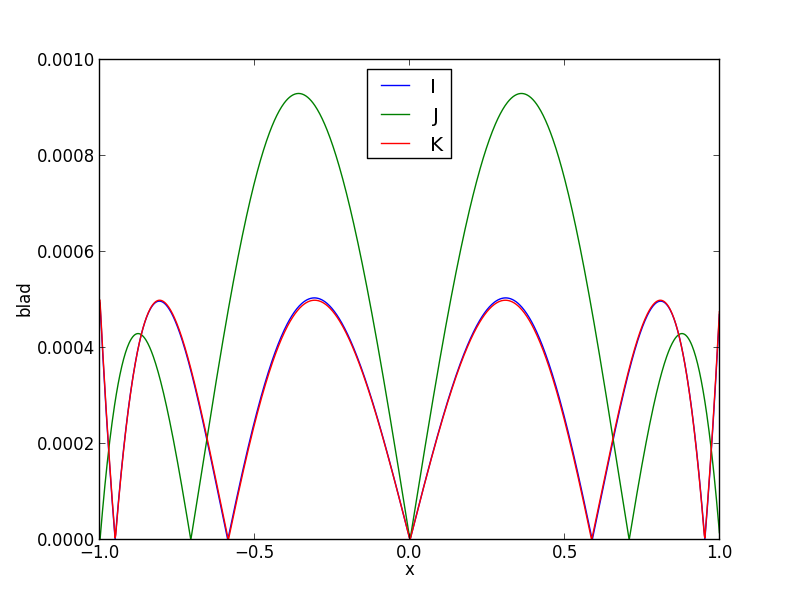
\includegraphics{graph1_4.png}
        \caption{Błąd bezwględny aproksymacji $\sin x$ dla $n=4$}\label{G:Wykressin4}
    \end{center}
    \end{figure}
\end{center}
\begin{center}
    \begin{figure}[!ht]
        \begin{center}
        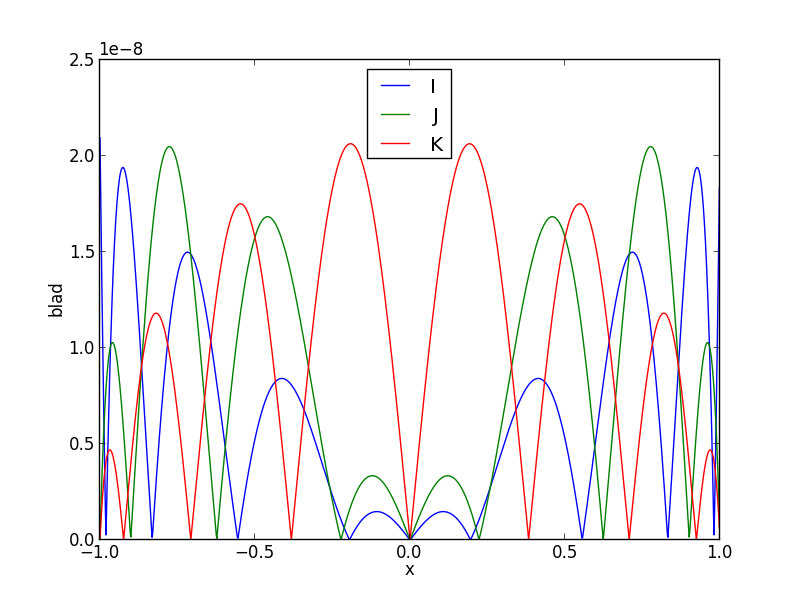
\includegraphics{graph1_7.png}
        \caption{Błąd bezwględny aproksymacji $\sin x$ dla $n=7$}\label{G:Wykressin7}
    \end{center}
    \end{figure}
\end{center}
\begin{center}
    \begin{figure}[!ht]
        \begin{center}
        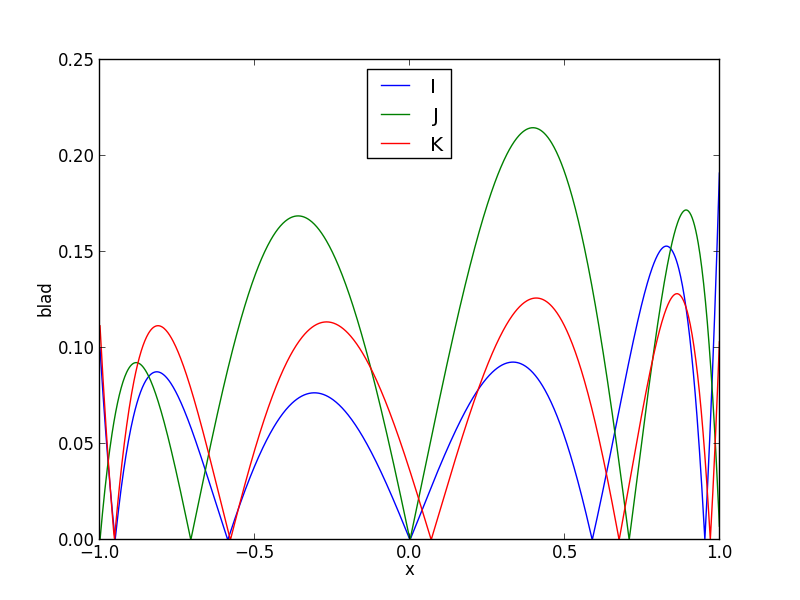
\includegraphics{graph2_4.png}
        \caption{Błąd bezwględny aproksymacji $x + 18x^2 + 2x^3 + 0.66x^5 + 0.167x^8 + 0.5x^9 + 0.125x^{10}$ dla $n=4$}\label{G:Wykrespoly4}
    \end{center}
    \end{figure}
\end{center}
\begin{center}
    \begin{figure}[!ht]
        \begin{center}
        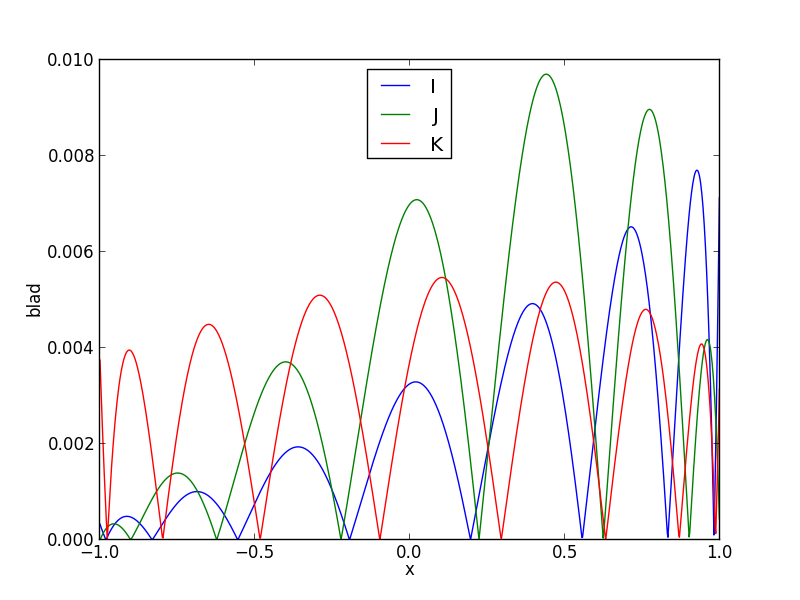
\includegraphics{graph2_7.png}
        \caption{Błąd bezwględny aproksymacji $x + 18x^2 + 2x^3 + 0.66x^5 + 0.167x^8 + 0.5x^9 + 0.125x^{10}$ dla $n=7$}\label{G:Wykrespoly7}
    \end{center}
    \end{figure}
\end{center}
\end{document}
